\section{Introduction}
\subsection{Terminology}
\begin{description}
	\item[Block access] 
		An access to a block of secondary storage. Since accessing secondary storage
		presents itself as the bottleneck in database latency, the time complexity of
		database operations is often represented by the number of block accesses rather
		than the number of RAM operations.
    \item[Data client]
    	A person or party collecting data for the puposes of learning analytics.
    \item[Data subject]
    	A person who contributes data to or is the subject of a learning analytics 
    	application. In the context of the survey tool, this is the person who
    	responds to a survey.
    \item[Learning management system]
	    A content management system, specifically designed for e-learning applications.
	    Examples of LMSs are Moodle and OLAT.
    \item[Learning record store]
    	A database system, possibly including analysis and visualization capabilities, 
	    for storing data of interest to learning analytics applications.
	    In the context of this thesis, LRS particularly refers to a system for storing and analyzing xAPI statements.
    	Examples for LRS systems are the TLA facts engine an HT2Labs's Learning Locker \cite{ht2labs-learninglocker}.
    \item[Survey item]
    	An organizational unit of a survey. In the context of this thesis,
    	a survey item may either be an entire questionnaire, a
    	dimension of a questionnaire or a single question. 
    \item[Tool provider]
	    In the context of LTI, the term \textit{tool provider} is used to describe a
	    system which provides an external tool to an LMS, thereby extending the capabilities of the LMS.
\end{description}

\subsection{Previous Work}
    As part of the computational humanities seminar, which was held by \profhd in winter 2017/18, Hannes Leutloff
    and I were tasked to digitize the evaluation framework for learning analytics (EFLA) \cite{efla} and to
    develop an online platform where the survey could be taken.

    \begin{figure}
        \centering
        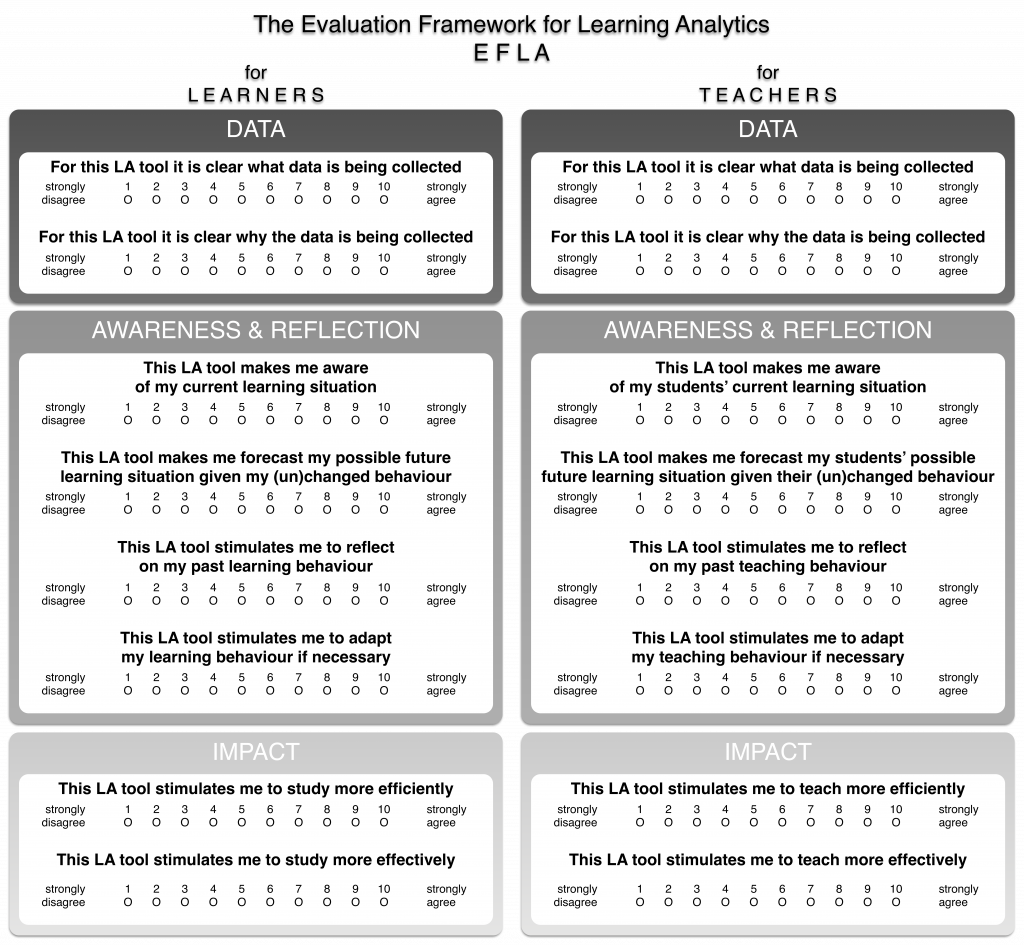
\includegraphics[width=\textwidth]{EFLA--greyscale}
        \caption{Template for the EFLA survey \cite{efla-website}}
        \label{fig:efla-template}
    \end{figure}

   The result is an online survey platform, where surveys similar to the EFLA can be created
   and hosted. While it is possible to create arbitrary survey items, some restrictions
   specific to the EFLA use-case apply (for a full list of features see table \ref{table:v1-features}).
   The original version of the survey tool is written in Python 3 and JavaScript for the server
   and user interface respectively. To be able to re-use code, the choice of language did not
   change with the new version.
   

   \begin{figure}
       \begin{tabularx}{\textwidth}{|l|X|}
            \hline
            Feature & Description \\
            \hline \hline
            Editable surveys & Edit titles, question texts and colors.\\
            Export to CSV & Export all results of a questionnaire to as CSV file\\
            Challenges & Validate data subject's email addresses. 
            White- and Blacklist email addresses. Protect surveys by password.\\
            Internationalisation & Survey items may have multiple translations.\\
            User accounts & Users may sign up and host surveys.\\
            Template surveys & Choose from a fixed set of template surveys.\\
            Visualisation & View survey results as a box plot.\\
            \hline
       \end{tabularx}
       \caption{Features of the previous version of the survey tool}
       \label{table:v1-features}
   \end{figure}

   \subsubsection{Data Model}

   \begin{figure}[H]
        \centering
        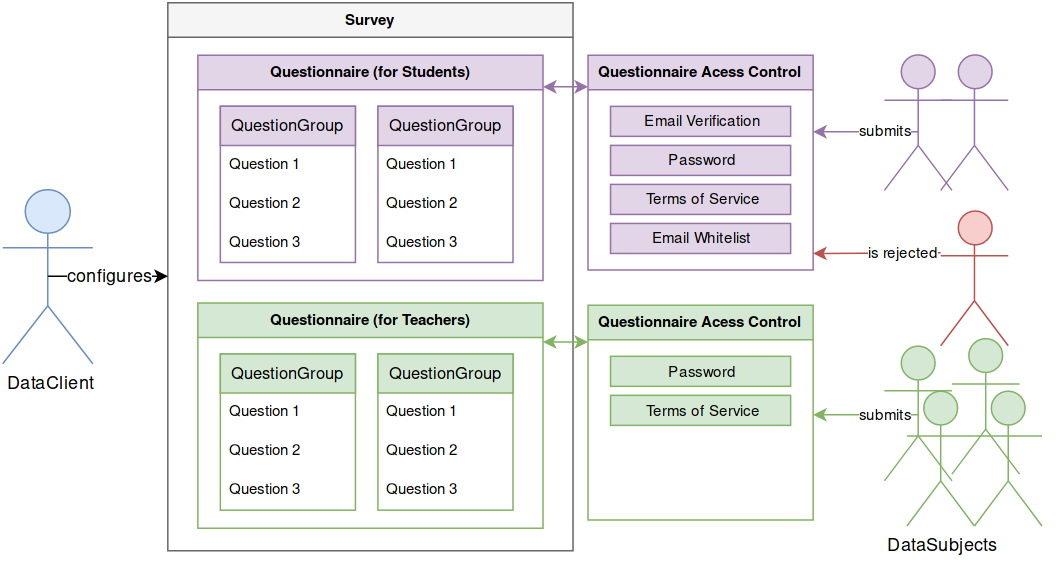
\includegraphics[width=\textwidth]{v1-model}
        \caption{Data model of the previous version}
        \label{fig:v1-data-model}
    \end{figure}

    \begin{wrapfigure}{o}{.5\textwidth}
        \centering
        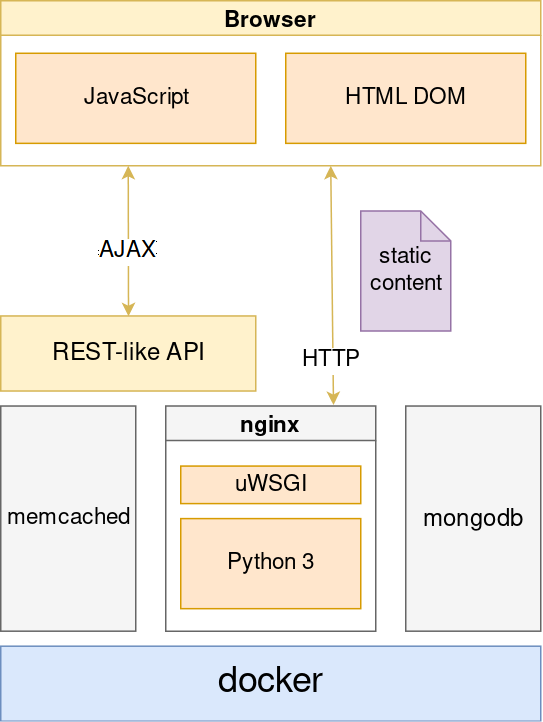
\includegraphics[width=0.4\textwidth]{v1-stack}
        \caption{Architecture overview of the previous version}
        \label{fig:v1-stack}
    \end{wrapfigure}

    The data model for the previous version is closely coupled to the specific needs of the
    EFLA survey, where a single survey consists of two questionnaires, targeting
    learners and teachers respectively.
    Each questionnaire controlls DataSubjects' rights to submit by it's own set of access 
    control modules, so that audience groups can be discriminated.
    Each questionnaire contains one or more question groups, which contains of
    one or more questions.

    \subsubsection{Architecture}

    The architecture for the previous version follows a simple client-server paradigm, where
    a web browser takes the role of the client. The server software consists of an
    application server, responding to API requests, a database and an in-memory
    key-value store for storing session data. There are two different user interfaces,
    one for data clients and one for data subjects. The data subjects' user interface
    is the page, where the survey is filled out and submitted. This page is rendered
    on the server using a templating engine and sent to the browser as a static HTML document.
    The user interface for data clients presents the user with an editor, where survey content
    can be created and modified. This user interface is realised as a one-page
    javascript application and was developed by Hannes Leutloff. Deployment is handled through
    Docker, with the help of the docker-compose tool.

\subsection{The TLA infrastructure}
    Prof. H. Drachsler's work groups' current efforts are targeted towards the implementation
    of a trusted learning analytics (TLA) infrastructure. This infrastructure will
    provide big data storage and analysis capabilities while complying with the european general
    data protection regulation (GDPR). A central part of this infrastructure are data
    providers. These data providers are tools which collect data and publish it to
    the TLA facts store, using the xAPI statement format as a common data representation.
    The aim is to not only create the infrastructure to collect and analyse data,
    but also to build and ecosystem of external tools and data providers
    which interface with TLAs core components.

\subsection{Goal}
    The goal of this thesis is to extend the functionality of the already existing
    survey tool and to contribute to the TLA ecosystem by integrating the
    survey tool as a data provider.

\subsection{Motivation}
    Online survey tools are not a new invention by any stretch of the imagination.
    An online search yields dozens of already existing survey platforms, both
    commercial and free to use. Some of the biggest competitors in this business
    are compared in table \ref{table:competitors}. For most use cases, one
    of the existing solutions will be sufficient. The survey tool described here
    aims at solving a unique challenge not solved by any competitor the author
    is aware of. This challenge is integration with Moodle and the TLA
    infrastructure for use at the Goethe University in Frankfurt Main.
    Features needed for this integration are single sign on, i.e.
    automated authentication of survey participants between Moodle and
    the survey tool, support for embedding via the LTI protocol, 
    as well as support for xAPI as a data exchange protocol.
    These requirements are discussed in greater detail in the Section
    ``Requirements Analysis''. While most survey providers, provide single
    sign on features, most only provide these capabilities to enterprise
    customers. Also, only one of the competitors looked at in this thesis
    supports CAS as a mechanism for this. None of the competitors
    supports data export as xAPI statements out of the box and require either
    manual programming for every survey or data conversion after export. 
    Out of the listed competitors, only one supports the LTI protocol for
    embedding the survey into Moodle and the only documentation of this 
    feature is an online video \ref{qualtrics-lti-video}. For these
    reasons, an alternative survey tool was developed.

    \begin{landscape}
        \begin{table}
            \begin{tabularx}{1.4\textheight}{|c|X|X|X|X|X|}
                \hline
                \diagbox{Feature}{Provider} & Google Forms & SurveyMonkey & QuestionPro & qualtrics & survey gizmo \\
                \hline 
                SSO & For managed accounts in G-Suite via SAML and LDAP \ref{googleforms-sso}
                    & Supported, but further information is only provided to potential customers. \ref{surveymonkey-sso}
                    & Through SAML and HMAC-SHA1 \ref{questionpro-sso}
                    & Through CAS, LDAP or SAML \ref{qualtrics-sso}
                    & Through SAML \ref{surveygizmo-sso} \ref{surveygizmo-sso2}
                    \\ \hline
                xAPI & Not supported, but has limited support for programmable event handlers. \ref{googleforms-webhooks}
                     & Not supported, but supports polling of survey results through an API. \ref{surveymonkey-api}
                     & Not supported, but has support for web hooks. \ref{questionpro-webhooks}
                     & Not supported, but supports polling of survey results through an API. \ref{qualtrics-api}
                     & Not supported, but has limited support for web hooks. \ref{surveygizmo-webhooks}
                     \\ \hline
                LTI & Unsupported 
                    & Unsupported 
                    & Unsupported
                    & Alledged experimental support, no official documentation exists. 
                    & Unsupported
                    \\
                \hline
            \end{tabularx}
            \caption{Comparison of survey providers}
            \label{table:competitors}
        \end{table}
    \end{landscape}

\subsection{Scope}
\label{section:introduction:scope}

    In this thesis, the overall structure of the survey platform and the server-side
    software stack, which was designed and developed by Noah Hummel is discussed.
    Implementational details are discussed only if they are central to the workings
    of the software, or solve a particular conceptual challenge.
    The user interface was designed and mainly developed by Hannes Leutloff, and
    is therefore not discussed in this thesis.
